% chktex-file 44

\newpage
\section{Benchmarking}\label{sec:benchmark}

This project uses benchmarking to determine the overall performance and scalability of the application, whilst also being useful in discovering any bottlenecks or bugs.
\x
To ensure consistency in these results, I've included the following constraints:

\begin{itemize}
  \item All benchmarks should be ran on the same hardware using the same OS,
  \item All tests should be ran three times,
  \item Test data should be pseudo-random, and
  \item All projects should aim for the target size of 40GB to match the average game size given in Section~\ref{subsec:design-data}.
\end{itemize}

\subsection*{Number of Peers}

For each run, we will create a project with 500 files, each of size 80MB and a shard size of 4MiB. We will then run $N$ peers locally to simulate a perfect network connection.


\begin{table}[ht]
  \vspace{-5mm}
  \begin{minipage}[t]{.5\textwidth }
    \vspace{-36mm}
    \begin{longtable}{l|llll|}
      \cline{2-5}\cline{2-5}\cline{2-5}\cline{2-5}\cline{2-5}
      & \multicolumn{4}{c|}{\hdr{Runtime (s)}}\\ \hline
      \multicolumn{1}{|l|}{\hdr{Peers}} 
      & \multicolumn{1}{l|}{\hdr{1}} 
      & \multicolumn{1}{l|}{\hdr{2}} 
      & \multicolumn{1}{l|}{\hdr{3}} & \hdr{avg.}  \\ \hline
      \multicolumn{1}{|l|}{1} & 
      \multicolumn{1}{l|}{1,513} & 
      \multicolumn{1}{l|}{1,511} & 
      \multicolumn{1}{l|}{1,511} &  
      1,512
      \\ \hline
      \multicolumn{1}{|l|}{2} & 
      \multicolumn{1}{l|}{777} & 
      \multicolumn{1}{l|}{775} & 
      \multicolumn{1}{l|}{777} &  
      776
      \\ \hline
      \multicolumn{1}{|l|}{4} & 
      \multicolumn{1}{l|}{397} & 
      \multicolumn{1}{l|}{397} & 
      \multicolumn{1}{l|}{396} &  
      397
      \\ \hline
      \multicolumn{1}{|l|}{8} & 
      \multicolumn{1}{l|}{227} & 
      \multicolumn{1}{l|}{223} & 
      \multicolumn{1}{l|}{224} &  
      225
      \\ \hline
      \caption{Raw data from peer count benchmark}
      \label{tab:bench-peer-count}
    \end{longtable}
  \end{minipage}%
  \begin{minipage}[t]{.5\textwidth}
      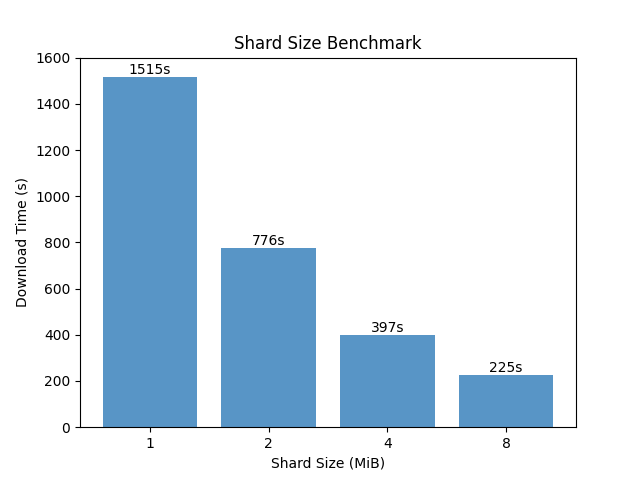
\includegraphics[width=\textwidth]{assets/images/charts/peer-count.png}
      \caption{Graphical version of Table~\ref{tab:bench-peer-count}}
  \end{minipage}
\end{table}

\vspace{-4mm}\noindent
This result shows us that we can massively increase the download speed by increasing the number of peers we are connected to. This shows that my application can correctly handle many concurrent peers \reqref{F-M7} and uses the increased connections to boost performance \reqref{NF-S1}.

\subsection*{Game Size}

For each run, we will create a project of $F$ files of size $S$MB, such that $F\times S = 40GB$. We will download the game off of 4 peers that are running locally on the same machine.

\begin{longtable}{rr|llll|}
  \hline
  \multicolumn{2}{|c|}{\hdr{File}}
  & \multicolumn{4}{c|}{\hdr{Runtime (s)}}
  \\\hline
  \multicolumn{1}{|l|}{\hdr{Count}} 
  & \hdr{Size (MB)}
  & \multicolumn{1}{l|}{\hdr{1}} 
  & \multicolumn{1}{l|}{\hdr{2}} 
  & \multicolumn{1}{l|}{\hdr{3}} 
  & \hdr{avg.}
  \\ \hline
  \multicolumn{1}{|r|}{200} 
  & 200
  & \multicolumn{1}{l|}{} 
  & \multicolumn{1}{l|}{} 
  & \multicolumn{1}{l|}{} 
  &  
  \\\hline
  \multicolumn{1}{|r|}{100} 
  & 400
  & \multicolumn{1}{l|}{} 
  & \multicolumn{1}{l|}{} 
  & \multicolumn{1}{l|}{} 
  & 
  \\\hline
  \multicolumn{1}{|r|}{50} 
  & 800
  & \multicolumn{1}{l|}{} 
  & \multicolumn{1}{l|}{} 
  & \multicolumn{1}{l|}{} 
  & 
  \\\hline
  \multicolumn{1}{|r|}{25} 
  & 1,600
  & \multicolumn{1}{l|}{} 
  & \multicolumn{1}{l|}{} 
  & \multicolumn{1}{l|}{} 
  & 
  \\\hline
  \multicolumn{1}{|r|}{5} 
  & 8,000
  & \multicolumn{1}{l|}{} 
  & \multicolumn{1}{l|}{} 
  & \multicolumn{1}{l|}{} 
  & 
  \\\hline
  \multicolumn{1}{|r|}{1} 
  & 40,000
  & \multicolumn{1}{l|}{} 
  & \multicolumn{1}{l|}{} 
  & \multicolumn{1}{l|}{} 
  &  
  \\\hline
  \caption{How varying file count and size affects download speed}
\end{longtable}

\noindent From these results, we can see that distributing data across a larger pool of files results in a greater download speed.
This occurred for several reasons:

\begin{enumerate}
  \item A file can only be written to by one process at one time so having less files will reduce the potential for parallelisation.
  \item For each block downloaded: we open a writer to a file, write a single block, and close the writer. This adds a lot of overhead for files that have many blocks.
\end{enumerate}